   \chapter{Experimentos e Resultados}
    \label{chap:experimentos}
   \section{Base de Imagens}
    \label{chap:basedeimagens}
   
   Os vídeos aplicados nos experimentos foram obtidos a partir do banco FISHCV155V, desenvolvido pelo grupo INOVISÃO da UCDB, em parceria com o IFMS e a empresa Projeto Pacu  \cite{Junior2019UFMS}. Os vídeos foram gravados entre os meses de julho e setembro de 2018 com uma câmera com resolução full hd ($1920\times1080$ pixels) e uma taxa de captura de 30 quadros por segundo. A câmera foi acoplada a uma estrutura criada pelos autores com uma inclinação aproximada de 12 graus, por onde os alevinos deslizam com o auxílio de água. A Figura \ref{Estrutura} mostra a estrutura construída para a obtenção dos vídeos.
   
   \begin{figure}
	\noindent\makebox[\textwidth]{%
		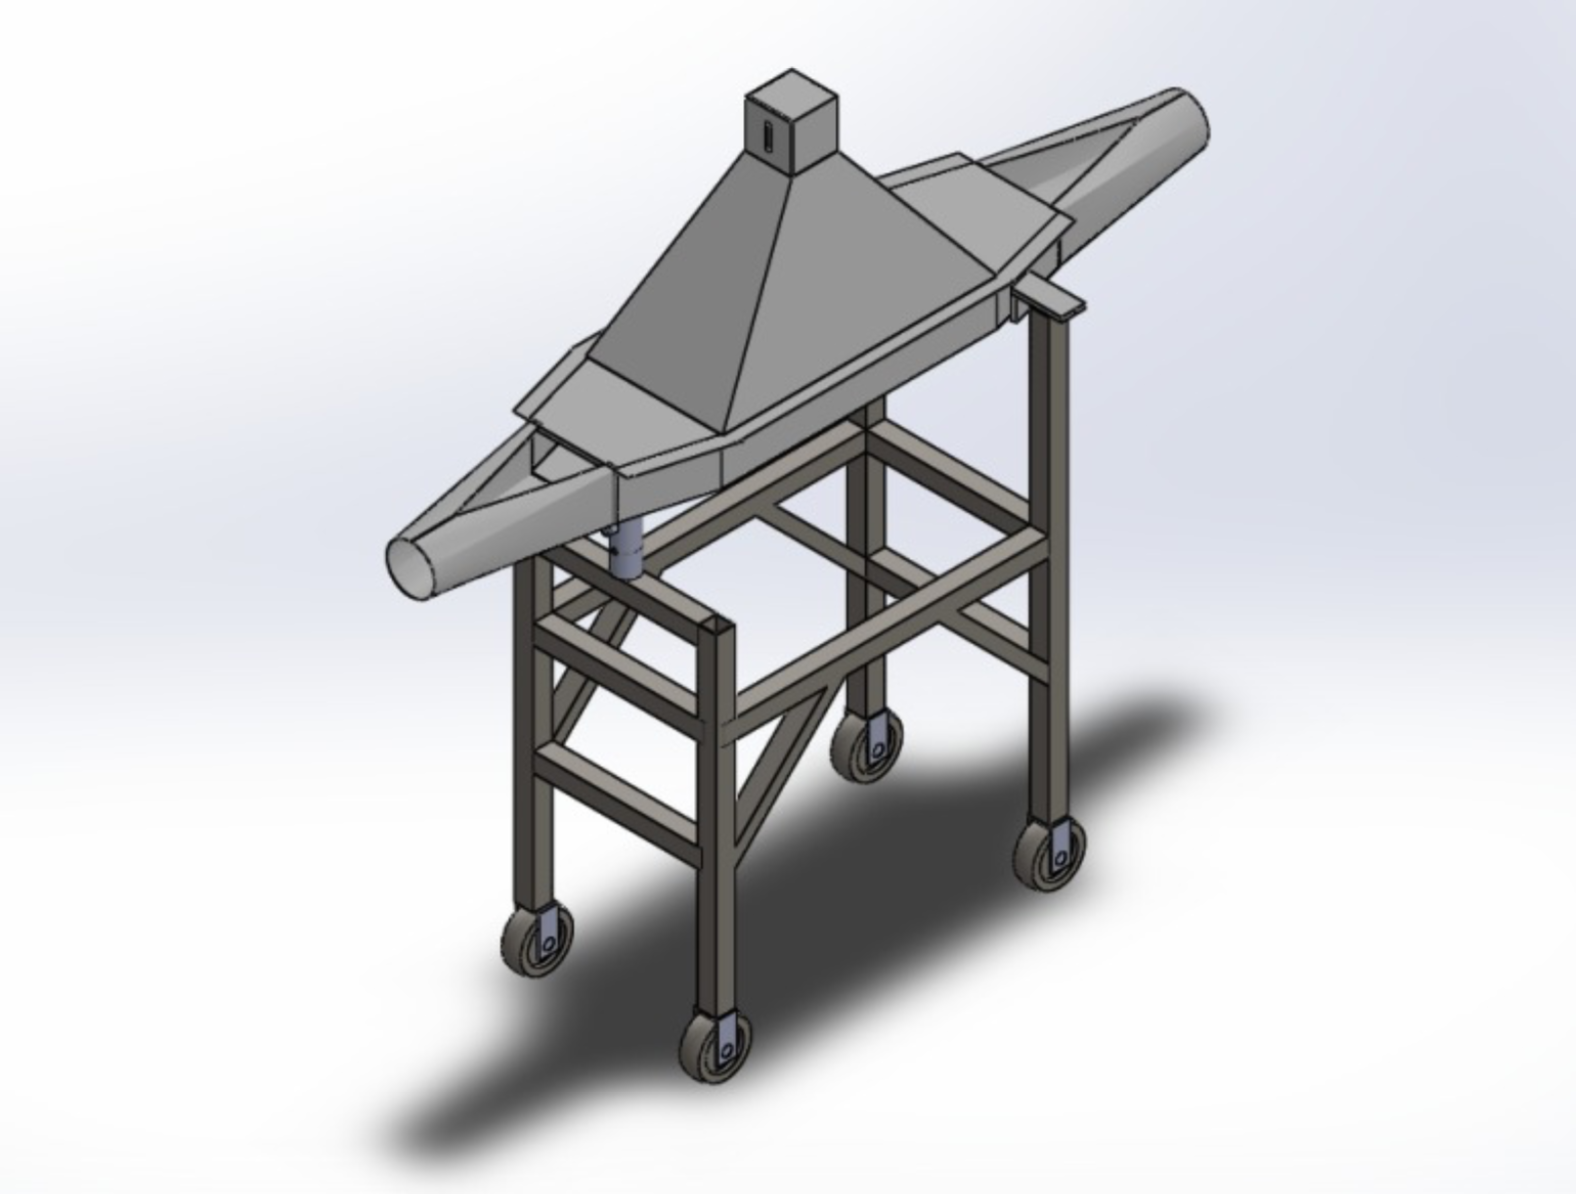
\includegraphics[width=0.5\textwidth]{image/estruturaCaptura.png}}
	\caption{Suporte para Captura das imagens proposta por \cite{Junior2019UFMS}}
	\label{Estrutura}
    \end{figure}
   
   Dentre os vídeos do banco de dados FISHCV155V, foram selecionados aleatoriamente 15 para compor o banco de dados do experimentos.
   O conjunto de treinamento é composto por 7 vídeos, sendo que o menor (tempo) vídeo contém 180 quadros e o maior 750 quadros; O conjunto de testes possui 4 vídeos, entre 240 e 300 quadros. %o menor contém 240 quadros e o maior contém 300; 
   O conjunto de validação possui 4 vídeos, sendo o menor 210 quadros e o maior 390. Na Figura \ref{Train} temos alguns exemplos das imagens utilizadas nos experimentos.
   Na Tabela \ref{tab:separation} a quantidade exata do conjunto é apresentado.
   
    \begin{table}[htb]
	\centering	
	\begin{tabular}{|p{2.7cm}|c|c|}
		\hline
		\multirow{2}{\linewidth}{\centering \textbf{Banco de Dados}} & \multicolumn{2}{|c|}{\textbf{Quantidades}} \\
    	\cline{2-3}
    	  & \textbf{Vídeos} & \textbf{Quadros} \\
		\hline
		Treinamento & $7$ & $2730$\\
		\hline
		Teste & $4$ & $1080$ \\
		\hline
		Validação & $4$ & $1230$ \\
		\hline
	\end{tabular}
	\caption{\label{tab:separation} Separação dos vídeos e quadros para os Experimentos}.
    \end{table}

   \begin{figure}[htb]
		\centering
		%\textbf{SEGNET SEM PONDERAÇÃO - OLHO DE RÃ} \\
		\subfloat{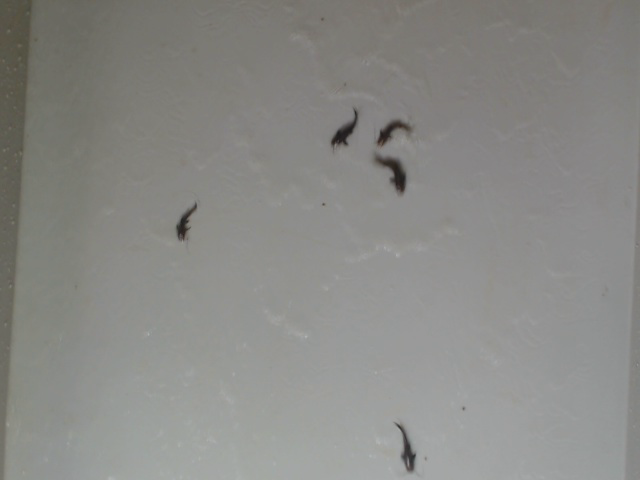
\includegraphics[width=.32\columnwidth]{image/Train/VID15_frame000222.png}}
		\hspace{.1cm}
		\subfloat{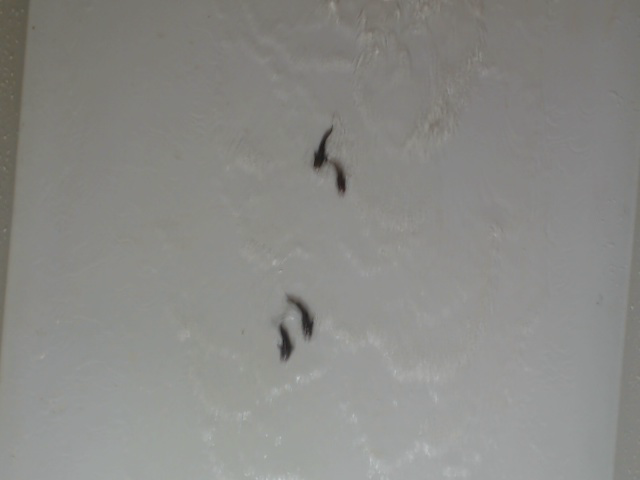
\includegraphics[width=.32\columnwidth]{image/Train/VID18_frame000244.png}}
		\hspace{.1cm}
		\subfloat{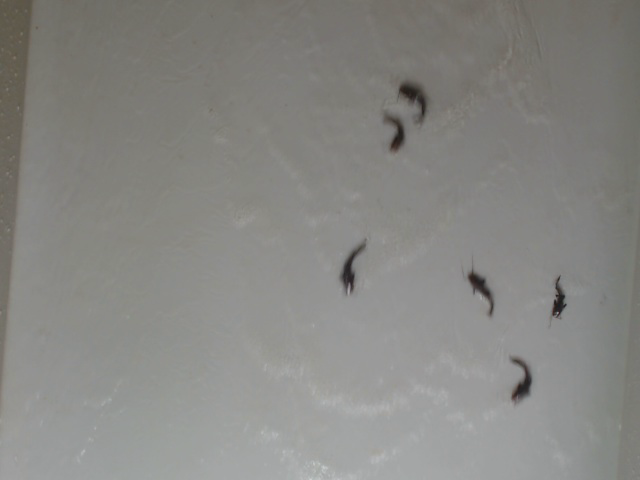
\includegraphics[width=.32\columnwidth]{image/Train/VID19_frame000313.png}}
		\hspace{.1cm}
		\caption{Imagens retiradas do conjunto de Treinamento \cite{Junior2019UFMS}.} % caption for whole figure
		\label{Train}
	\end{figure}
	


\subsection{Configuração dos Experimentos}

Para avaliar a abordagem proposta, as amostras foram divididas aleatoriamente em conjuntos de treinamento contendo 7 vídeos, validação 4 vídeos e teste 4 vídeos.
Para o treinamento, o otimizador Gradiente Descendente Estocástico foi usado com um momento de 0,9.
O ajuste de hiper parâmetros na taxa de aprendizado e no número de épocas foi realizado usando o conjunto de validação para reduzir o risco de \textit{overfitting}.
Após experimentos preliminares para ajuste de hiper parâmetro, a taxa de aprendizado foi de 0,01 e o número de épocas foi de 100.

Todos os experimentos foram executados na GPU (Unidade
de Processamento Gráfico) NVIDIA GeForce GTX TITAN X (5120 Compute Unified Device Architecture - núcleos CUDA e memória gráfica de 12 GB ), sistema operacional Ubuntu 18.04. A implementação proposta faz o uso da API (Interface de Programação de Aplicativos) de alto nível denominada Keras \cite{chollet2015keras}, escrita na linguagem de programação Python. As rotinas desta interface são executadas através da biblioteca de código aberto TensorFlow \cite{tensorflow2015-whitepaper}.

\subsubsection{Transfer Learning}
Em vez de treinar a abordagem proposta do zero, os pesos da primeira parte foram inicializados com pesos pré-treinados no ImageNet em um conceito conhecido como \textit{transfer learning}.
Esse método proporciona uma certa rapidez no treinamento de CNNs, evitando treinamentos do zero (aleatoriamente). 
Quanto maior e mais geral o conjunto de treinamento do modelo pré-treinado, maior será a eficiência da transferência de aprendizado (\cite{tensorflow2015-whitepaper,c231stan}). 
A ImageNet é um conjunto que contém 1,2 milhões de imagens com 1000 categorias \cite{DBLP:journals/corr/RussakovskyDSKSMHKKBBF14}. Por ser um conjunto extenso existem vários modelos treinados nas arquiteturas mais conhecidas da literatura.

\subsubsection{Métricas de Classificação}
%\paragraph{MAE}
Para avaliar o método foram utilizados as métricas de regressão que medem a concordância entre o número de objetos anotados e os preditos. A métrica de erro absoluto médio (\textit{mean absolute error} - MAE) é calculada conforme a Equação \ref{eq:MAE}.

\begin{equation}
\label{eq:MAE}
    MAE = \frac{\sum^{T}_{t=1}{|\hat{x}_t-{x}_t|}}{T}
\end{equation}
onde $\hat{x}_t$ representa o número de objetos preditos pelo método e ${x_t}$ o número de objetos anotados em um conjunto de $T$ quadros do conjunto de testes \cite{MAE}. 

%, erro quadrático médio (\textit{mean squared error} - MSE) 
%,coeficiente de determinação ($R^2$) e erro quadrático médio da raiz normalizado (\textit{normalized root-mean-squared error} - NRMSE).

Para avaliar a localização dos objetos preditos em uma imagem, nós usamos a precisão, revocação e métrica F1 ou medida-f.
Para calcular essas métricas, é necessário determinar o número de verdadeiros positivos (VP), falsos positivos (FP) e falsos negativos (FN).
Um verdadeiro positivo é obtido se um ponto predito pelo método proposto está dentro de um raio máximo $r$ de um ponto rotulado (neste trabalho usamos raio máximo igual a 5 pixels).
Um falso positivo é obtido quando o método proposto prediz um objeto que não foi rotulado, isto é, nenhum ponto a uma distância $r$.
Por fim, um falso negativo é obtido quando nenhum ponto é predito a uma distância $r$ de um ponto rotulado.

A Precisão é definida conforme a Equação \ref{eq:precision}, isto é, o número de verdadeiros positivos (VP) sobre o número de verdadeiros positivos mais o número de falsos positivos (FP).

\begin{equation}
\label{eq:precision}
    P = \frac{VP}{VP+FP}
\end{equation}

Revocação é definido com o número de verdadeiros positivos (VP) sobre o número de verdadeiros positivos mais o número de falsos negativos (FN), conforme a Equação \ref{eq:recall}.

\begin{equation}
    \label{eq:recall}
    R = \frac{VP}{VP+FN}
\end{equation}

Para obter uma exatidão dos acertos, usamos a F1 que produz uma média harmônica da precisão e da revocação. A revocação está focada nos pontos que deverão ser classificados como positivos, enquanto que a precisão calcula os pontos positivos que foram preditos como positivos pelo modelo. A função alcança seu melhor valor em 1 e pior em 0 \cite{f1}: 
\begin{equation}
    F1 = 2 \cdot \frac{P\cdot R}{P + R}
\end{equation}

